\documentclass{standalone}

\usepackage{tikz}
\usetikzlibrary{arrows}
\usetikzlibrary{decorations.markings}

\begin{document}

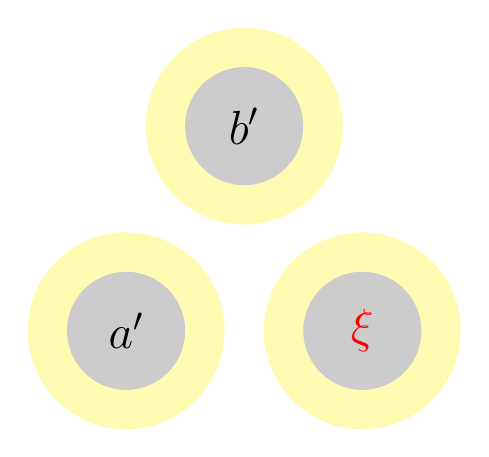
\begin{tikzpicture}

  \draw[opacity=.3,line width=25mm,line cap=round,draw=yellow] (1.5, 2.6) -- (1.5, 2.6);
  \draw[opacity=.3,line width=25mm,line cap=round,draw=yellow] (0, 0) -- (0, 0);
  \draw[opacity=.3,line width=25mm,line cap=round,draw=yellow] (3, 0) -- (3, 0);

  \node (a) [style={minimum size=1.5cm,fill=black!20!white,text=black,shape=circle}] at (0, 0) {\LARGE{$a'$}};
  \node (b) [style={minimum size=1.5cm,fill=black!20!white,text=black,shape=circle}] at (1.5, 2.6) {\LARGE{$b'$}};
  \node (xi) [style={minimum size=1.5cm,fill=black!20!white,text=black,shape=circle}] at (3, 0) {\textcolor{red}{\LARGE{$\xi$}}};
\end{tikzpicture}

\end{document}
